\section{Architektura aplikacji}

Aplikacja egzaminująca model składa się z dwóch warstw - części GUI i części serwerowej. Część serwerowa odpowiedzialna jest za całościową analizę reguł, oraz generowanie kodu. Jest ona napisana w technologii Spring Boot, w języku Kotlin. Warstwa GUI stworzona została przy użyciu biblioteki Angular. Komunikacja pomiędzy obydwoma częściami odbywa się przy pomocy serwisów REST. 

Z punktu widzenia użytkownika aplikacja składa się z trzech wyraźnie wyodrębnionych części

\begin{enumerate}
	\item Sekcji danych wejściowych
	\item Sekcji wyników analizy NLP
	\item Sekcji wygenerowanego kodu
\end{enumerate}


\subsection{Sekcja danych wejściowych}
W tej części aplikacji użytkownik może zarządzać danymi, jakie poddawane są analizie NLP. Interfejs aplikacji umożliwia dodawanie nowych reguł, modyfikację treści istniejących, oraz kasowanie reguł. 
\begin{figure}[H]
	\centering
	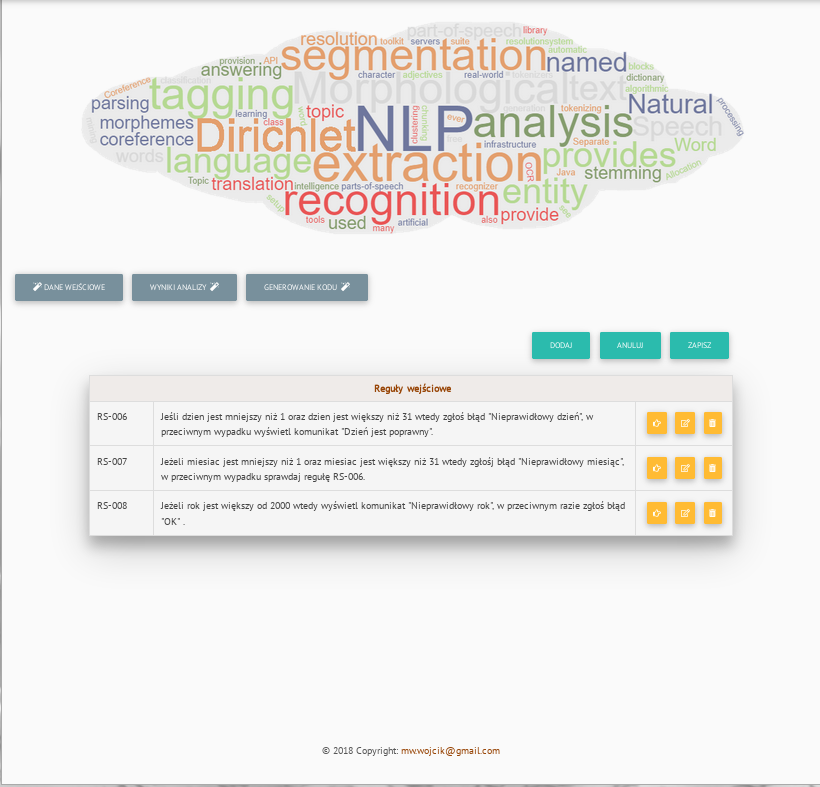
\includegraphics[scale=0.7]{img/app/app-we.png}
	\caption{Główne okno aplikacji - sekcja definicji reguł wejściowych}\label{app-ekran-we}
\end{figure}
\subsection{Sekcja prezentacji wyników analizy NLP}
Ten ekran jest nieco ciekawszy od poprzedniego. Prezentuje wyniki analizy reguł wykonanej w
oparciu o algorytmy uczenia maszynowego dostępne w ramach biblioteki \textit{OpenNLP}.
Wyniki analizy prezentowane są w tabelach według następującego schematu:

\begin{enumerate}
	\item \textbf{Reguła wejściowa} - informacja o treści reguły poddawanej analizie algorytmicznej.
	\item	\textbf{Wyodrębnione komunikaty} - jest to lista komunikatów użytkownika, które zostały odnalezione w regule.W celu uproszczenia przetwarzania sekwencji przez algorytmy NLP komunikaty są wyodrębniane i zastępowane
	słowem - markerem identyfikującym komunikat. Jako komunikat uznaje się ciąg znaków otoczonych znakiem podwójnego cudzysłowu.
	\item \textbf{Rozpoznane tokeny}-jest to tabela pokazująca wyniki działania algorytmu NLP. Prezentuje ona regułę rozbitą na pojedyncze tokeny.
	Przy każdym tokenie  wskazana jest logiczna encja, do której przyporządkował go algorytm dokonujący analizy, oraz liczbowe prawdopodobieństwo z jaką nastąpiło dopasowanie.
	Ostatnia kolumna tej tabeli ma zastosowanie tylko do wybranych bytów logicznych i służy do normalizacji tokenów. Np. tokeny "równy", "równa", "jest równy" należą do jednej wspólnej kategorii oznaczającej równość "==", a tokeny "jest większy lub równy", "jest nie mniejszy niż" oznaczają kategorię ">="
	\item \textbf{Rozpoznane parametry wejściowe}- w tabeli tej prezentowane są tokeny uznane jako parametry wejściowe do reguły. Zwykle występują one w wyrażeniach warunkowych.
	W przypadku gdy warunek reguły skonstruowany jest w taki sposób, że następuje porównanie z wartością stałą (np liczbową lub datę), wtedy taka wartość jest traktowana jako parametr wejściowy reguły z przypisaną wartością domyślną.
	Warunkiem poprawności analizy reguły jest właściwe przyporządkowanie typów danych do parametrów reguły. Jeśli nie uda się wnioskowanie automatyczne, to informacje te muszą być wprowadzone przez użytkownika w do drugiej kolumny tabeli parametrów.
	\item \textbf{Rozpoznane wywołania innych reguł}-W tabeli tej prezentowane są odnalezione odwołania do innych reguł,oraz mapowania parametrów wejściowych reguły wołającej i reguły wołanej.
\end{enumerate}
\paragraph
Prezentacja wyników następuje po wybraniu reguły z listy w panelu bocznym. Zielony znacznik świadczy o tym że dopełnione zostały wszystkie doprecyzowania i mapowania parametrów, więc aplikacja posiada komplet informacji potrzebnych do wygenerowania kodu.


\begin{figure}[H]
	\centering
	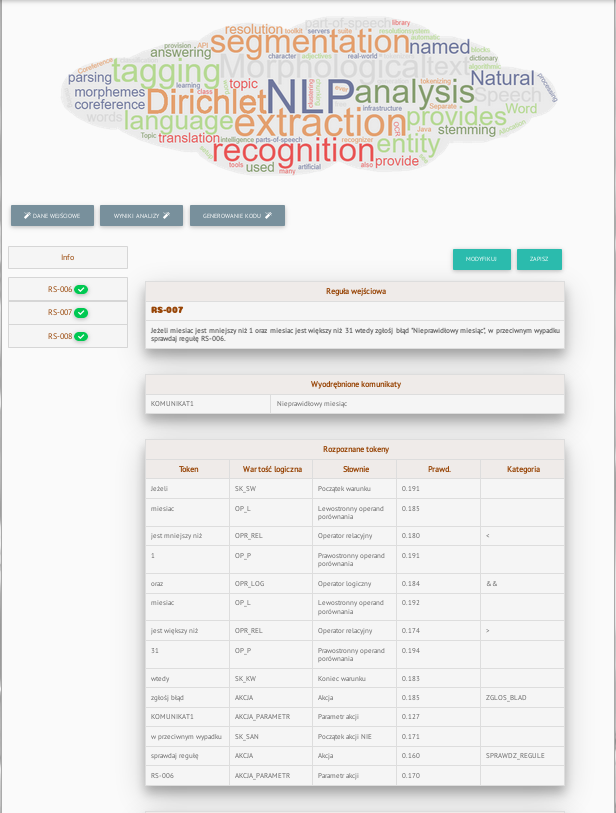
\includegraphics[scale=0.7]{img/app/app-reg.png}
	\caption{Główne okno aplikacji - sekcja analizy NLP}\label{app-ekran-wyniki}
\end{figure}

\subsection{Sekcja wygenerowanego kodu}
W trzeciej sekcji programu pokazany jest wynik przekształcenia reguły do kompilowalnego kodu \textit{Kotlin}. Dla każdej reguły tworzona jest osobna metoda. Nazwa metody jest tożsama z kodem reguły. Metoda przyjmuje parametry, które zaprezentowane są w tabeli ,,Parametry wejściowe'' na ekranie wyników analizy. 
\begin{figure}[H]
	\centering
	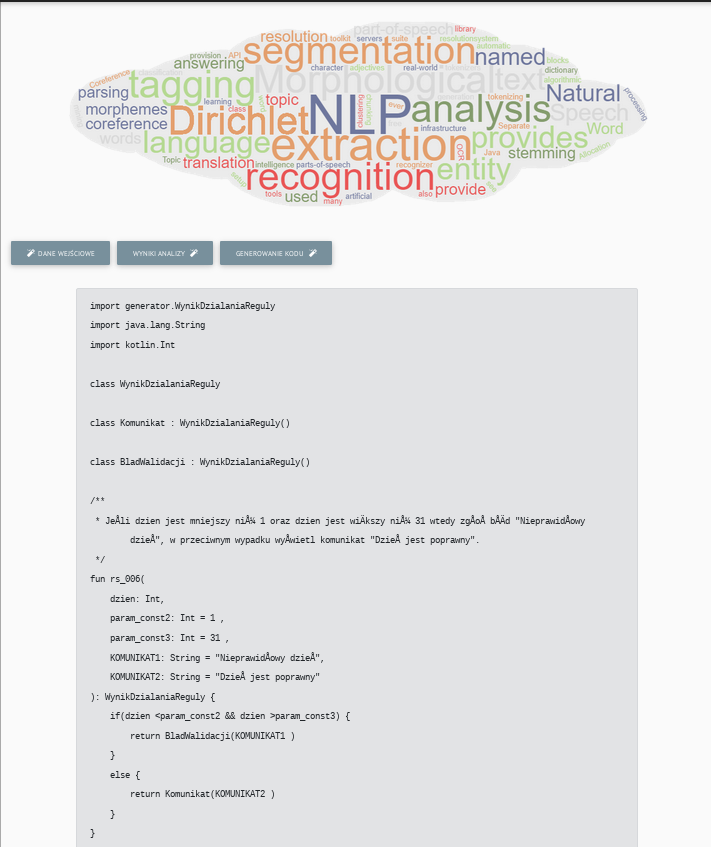
\includegraphics[scale=0.7]{img/app/app-kod.png}
	\caption{Główne okno aplikacji - sekcja wygenerowanego kodu}\label{app-ekran-kod}
\end{figure}

Uwaga! Sekcja ta jest dostępna tylko wtedy, gdy wszystkie reguły zaprezentowane na ekranie analizy danych \ref{app-ekran-wyniki} zostaną zwalidowane pozytywnie, czyli aplikacja uzyska wszystkie dane potrzebne do wygenerowania kodu.